\documentclass[12pt]{article} 
\usepackage[utf8]{inputenc}
\usepackage[T1]{fontenc}
\usepackage[french]{babel}
\usepackage{geometry} 
\geometry{a4paper} 

\usepackage{graphicx} 

\usepackage{float} 
\usepackage{wrapfig}

\linespread{1.2}

\setlength\parindent{2.5pt}

\graphicspath{{Pictures/}} 


\begin{document}
\begin{titlepage}
\newcommand{\HRule}{\rule{\linewidth}{0.5mm}}
\center 

\textsc{\LARGE Université de Lorraine}\\[1.5cm] 
\textsc{\Large Projet Tuteuré}\\[0.5cm]
\textsc{\large ASRALL}\\[0.5cm]

\HRule \\[0.4cm]
{ \huge \bfseries Systèmes de Fichiers Distribués}\\[0.4cm] 
\HRule \\[1.5cm]

\begin{minipage}{0.4\textwidth}
\begin{flushleft} \large
\emph{Author:}\\
Julien \textsc{SCHNEIDER}\\
Jean \textsc{LUTZ}\\
Yannick \textsc{LAPREVOTTE}\\
Ricardo \textsc{RODRÍGUEZ}\\
\end{flushleft}
\end{minipage}
~
\begin{minipage}{0.4\textwidth}
\begin{flushright} \large
\emph{Supervisor:} \\
 Stephane \textsc{CASSET} 
\end{flushright}
\end{minipage}\\[4cm]

{\large \today}\\[3cm] 

\vfill 
\end{titlepage}


\tableofcontents 

\newpage 

\section{Introduction}

La technologie avance à grands pas dans la société. Cette conclusion est bien connu de tous. En effet il suffit aujourd'hui de tourner la tête pour s'en rendre compte très facilement. La technologie de pointe à investi notre quotidien. Cette idée s'est  endurci depuis l'arrivée des smart phones et des tablettes qui ont fais avancer l'humanité d'un pas de plus vers la dépendance aux nouvelles technologies. Cette évolution est dû aux progrès techniques notamment en terme de nanotechnologies. En effet, la nanotechnologie permet des gravures et des soudures de plus en plus fines, de l'ordre du nanomètre, permettant d’accroître en continue la puissance de nos ordinateurs, comme le démontre la loi de Moore.

La croissance de la puissance de calcul permet aux développeurs d'envisager des programmes toujours plus puissants et plus complexes, ce qui va permettre de créer de nouvelles technologies, de nouveaux services , et donc de nouveaux besoins. C'est un de ces nouveaux besoins qui nous intéresse : le cloud computing. Celui-ci est né grâce à l'arrivée chez les particuliers d'un réseaux plus rapide (modem à adsl à fibre optique), mais aussi grâce à la baisse des prix des disques durs, et surtout, à l'arrivée des nombreux appareils nomades sophistiqués comme les tablettes, les smartphones... Le cloud permet de pouvoir sauvegardé des données sans risquer de les perdre (normalement). Mais l'idée principale est de pouvoir avoir accès à ces données depuis n'importe quel appareil via le réseau. En effet, l'utilisateur d'aujourd'hui veut à sa disposition toutes sa médiathèque même si les capacités de stockages ne le permettent pas sur tous ses appareils. Le cloud permet aussi le partage de documents entre un groupe de personnes. En 2014 le cloud computing est en pleine croissance, et cette tendance est loin de s'inverser, comme le prouve Google Chrome OS, le système d'exploitation de Google où toute application s'appuie sur le cloud computing. Ce système d'exploitation est un grand pas en avant et reflète l'avenir de l'informatique. C'est pourquoi, cette technologie très prometteuse est incontournable en tant qu'administrateur systèmes et réseaux. Mais comment fonctionne ces plate-formes, sur qu'elle technologie reposent elles ? 


En vérité, le cloud computing se pratique depuis longtemps, bien avant l'arrivée des smart phones. Seulement, le terme n'était pas le même car il s'utilisait d'une autre façon. Par exemple, l'utilisation d'une messagerie en ligne, donc avec les mails stockés sur un serveur distant, peut être considéré comme du clous. La connotation retenue, est celle d'un serveur de fichier. Il existe de nombreux programmes qui permettaient cela, comme NFS, (S)FTP... FTP ne permet que des connexions ponctuelles entre un serveur et un client, ce qui n'est pas très optimale et qui ne réponds plus aux besoins actuels. NFS se rapproche plus de notre technologie mais il pose de gros soucis. Le premier problème est son manque de sécurité, il est formellement déconseillé de l’utiliser publiquement sur le web. Ce protocole est préconisé d'être utiliser uniquement sur un LAN sécurisé. Son deuxième point faible est intégrité des données. En effet, la perte de données n'est absolument pas tolérable. Du RAID pourrait régler le problème, mais cette solution ne permet pas de répondre à la contrainte géographique. Un autre problème apparaît pour l'administrateur : avec l'effervescence du cloud computing, et la progression infinie de la masse de données totale dans le monde (bigdata), le stockage des données est une tâche extrêmement compliqué. Il faut donc un système flexible au maximum afin d'en faciliter la maintenance. NFS est incapable de fournir cette qualité de service exigée. C'est avec ce manque de moyens que sont apparus les systèmes de fichiers distribués. Ceph et Lustre, les deux systèmes qui nous intéressent, font parties de cette catégorie.

\subsection{Systèmes de Fichiers Distribué}
Deux notions se distinguent dans ce titre. La notion de système de fichier et le terme 'distribué'. 
	Un système de fichier c'est la couche du système qui va s'occuper de stocker/récupérer les données sur une mémoire secondaire, c'est à dire un disque dur, une clef usb, une disquette, un CD-ROM... Il existe des systèmes de fichiers journalisés et non journalisés. Un système de fichiers journalisés va enregistrer les données en cours d'opération en vue de garantir l'intégrité des données si la machine se coupe brutalement. Les FS ('File System' ou système de fichier en anglais) les plus répandus et les plus récents maintiennent majoritairement un journal. Il existe aussi des FS spécialisés pour le réseau comme NFS vu précédemment. Cependant, Lustre et Ceph présentent une caractéristique en plus.
	Nos deux systèmes de fichiers sont distribués. En d'autres mots, ils fonctionnent tous les deux avec plusieurs serveurs et plusieurs clients. Plus particulièrement, ces serveurs sont liés via un cluster. Cluster, ou grappe de serveurs, est une technologie qui consiste à réunir des serveurs (dans notre cas on peut parler de nœud) en un. Ainsi, cette grappe se partage toutes leurs ressources matérielles offrant de nombreux avantages comme faciliter la gestion des montées en charges. Un exemple très simple pour comprendre : des serveurs hébergeant un site web pour un fast food vont subirent des pics de requêtes aux alentours de midi et en fin d'après midi. Si ce fast food est implanté partout dans le monde, ses machines en Asie ne subiront pas en même temps que ceux en Europe à cause du décalage horaire. Cette entreprise a donc tout intérêt de lier ses serveurs via un cluster afin de pourvoir profiter toute la puissance de leur SI là où ils sont le plus sollicités à un moment donné. Un autre avantage de ce système de grappe est la forte disponibilité. En effet, il n'y a plus vraiment de goulot d'étranglement. Dans l'exemple précédent, si un pirate attaque le cluster par déni de service, il est obligé de faire tomber tous les serveurs pour rendre le service indisponible. La tâche devient donc très délicate pour l'attaquant. Les serveurs de Ceph et Lustre sont donc réunis en grappe. 
	Les systèmes de fichiers distribués ont aussi la particularité d'être capable de gérer des quantités énormes de données, de l'ordre du pétaoctet (1 million de Go) et sont souvent utilisés dans des data center. Il peut même être question de big data, c'est à dire la gestion de données de l'ordre du zettaoctet, 1 million de pétaoctets! Le big data est principalement présent en laboratoire, mais il ne peut que s'amplifier et il risque d'être beaucoup plus présent dans les entreprises dans un avenir proche. Il faut donc s'y préparé. C'est pourquoi les recherches sont très actives et ne risquent pas de s'estomper tout de suite.

\section{Ceph}
\subsection{Conclusion Ceph}
\newpage
\section{Lustre}
\begin{figure}[H] 
\center{
\includegraphics[width=0.5\linewidth]{placeholder}}
\caption{Lustre F.S.}
\label{fig:speciation}
\end{figure}

\subsection{Introduction}
Lustre est un système de fichiers distribué libre(sous licence GPL v2), utilisé pour de très grandes grappes de serveurs. Son nom vient de la combinaison de deux mots, «Linux» et «cluster». Le projet a commencé comme un projet de recherche en 1999 par Peter Braam, en 2007 Sun Microsystems a continué son développement, en 2010 avec l'acquisition de Sun Oracle a commencé à maintenir et sortir nouvelles versions de Lustre, en décembre du 2010 Oracle a arrêté le développement du système de fichiers version 2.x, plusieurs nouvelles organisations surgirent à fournir un soutien et de développement dans un modèle de développement communautaire ouvert, comprenant \textit{Whamcloud}, \textit{Open Scalable File Systems, Inc. (OpenSFS)}, \textit{EUROPEAN Open File Systems (EOFS)} et autres. En 2012 WhamCloud a été rachetée par Intel.\\


Lustre a la possibilité de accueillir des dizaines de milliers de systèmes client et une grande quantité de données, pétaoctets\footnote{Un pétaoctet contient \begin{math}10^{15}\end{math} octets} de stockage et des centaines de gigaoctets(Go) de débit Entrée/Sortie. 

\subsubsection{Les composants de Lustre}
\begin{description}
\item[Serveur de Métadonnées \textit{(Metadata Server «MDS»)}:]
Le serveur MDS rend les métadonnées, stockées dans un ou plusieurs MDT, disponibles pour des clients Lustre. Chaque MDS gère les noms et répertoires dans le systèmes de fichiers Lustre.
\item[Cible de Métadonnées \textit{(Metadata Target «MDT»)}:] Le MDT stocke les métadonnées(tels que les noms de fichiers, les répertoires et la structure des fichiers) sur un MDS. Chaque système de fichiers possède un MDT. Une MDT sur une cible de stockage partagé peut être disponible pour de nombreux MDS, bien que l'on devrait utiliser effectivement. Si une MDS actif échoue, un MDS passif peut servir le MDT et le rendre disponible aux clients. Ceci est appelé \textit{MDS failover}.
\item[Serveur de Stockage d'Objets \textit{(Object Storage Server «OSS»)}:]
L'OSS fournit un service d'Entrée/Sortie de fichiers et \textit{network request handling} pour un ou plusieurs OST locaux. Typiquement, un OSS sert entre 2 et 8 OST, jusqu'à 8 To\footnote{Un téraoctet contient \begin{math}10^{12}\end{math}octets.}
\item[Cible de Stockage d'Objets \textit{(Object Storage Target «OST»)}:]
L'OST stocke les données(des morceaux de fichiers de l'utilisateur) comme des objets de données sur un ou plusieurs OSS. Un seul système de fichiers Lustre peut avoir plusieurs OST, servant chacun un sous-ensamble de fichiers données. Il n'est pas nécessairement une correspondance 1:1 entre un fichier et un OST. Pour optimiser les performances, un fichiers peut être distribué sur plusieurs OST.
\item[Serveur de Gestion \textit{(Management Server «MGS»)}:]
Le MGS stocke les informations de configuration pour tous les systèmes de fichiers Lustre dans une grappe de serveurs. Chaque composent Lustre contacte le MGS pour fournir information, et les Lustre clients contactent le MGS pour obtenir information.
\item[Lustre clients:]Lustre clients sont noeuds exécutant le logiciel Lustre qui leur permet de monter le système de fichiers Lustre.

Le logiciel client de Lustre est composé d'une interface entre le \textit{Linux Virtual File System} et les serveurs Lustre. Chaque cible(composant de Lustre) a une contra partie client: Client de Métadonnées (MDC), Client de Stockage d'Objets(OSC) et un Client de Gestion(MGC). Un groupe de OSC sont intégrés dans un Volume d'objets logique(\textit{Logical Object Volume «LOV»}). Travaillant en collaboration, les OSC fournissent un accès transparent au système de fichiers.

Les clients qui montent le système de fichiers Lustre, voient un seul, cohérente, espace de noms(\textit{namespace}), synchronisé toujours. Différents clients peuvent écrire aux différentes parties d'un même fichier en même temps, tandis que d'autres clients peuvent lire le fichier.
\end{description}
\subsubsection{Principales Caractéristiques de Lustre}

Les principales caractéristiques de Lustre comprennent: \\

\begin{description}

\item[Évolutivité: ]
 Lustre échelles haut ou le bas par rapport au nombre de postes clients, stockage sur disque et bande passante. Actuellement , Lustre est en cours d'exécution dans des environnements de production avec un maximum de 26 000 postes clients, avec de nombreux grappes d'entre 10,000 et 20,000 clients. Autres installations fournissent Lustre d'espace de stockage en disque agrégé et bande passante allant jusqu'à 1000 OST fonctionnant sur plus de 450 OSS. Plusieurs systèmes de fichiers Lustre avec une capacité de 1 pétaoctet ou plus (permettant le stockage de jusqu'à 2 milliards de fichiers) ont été en usage depuis 2006.
\item[Performance: ]
 Lustre déploiements dans des environnements de production offrent actuellement la performance de jusqu'à 100 Go par seconde. Dans un environnement de test, une performance de 130 Go par seconde a été soutenue. Lustre seul débit de poste client a été mesurée à 2 Go par seconde (max) et OSS débit de 2,5 Go par seconde (max). Lustre a été exécuté à 240 Go par seconde sur le système de fichiers d'araignée(Spider File System) à Oak Ridge National Laboratories.

\item[Conformité POSIX:]Dans un cluster, la conformité POSIX signifie que la plupart des opérations sont atomiques et les clients ne voient jamais des données périmées ou métadonnées .
\item[Haute Disponibilité:]Lustre propose des partitions de stockage partagés pour les cibles de l'OSS (OST), et une partition de stockage partagé pour la cible MDS (MDT).

\item[Sécurité:]En Lustre, il s'agit d'une option pour les connexions TCP seulement de ports privilégiés. Manipulation des membres du groupe est basée sur le serveur. POSIX listes de contrôle d'accès (ACL) sont pris en charge .
\item[Open Source:] Lustre est sous licence GNU GPL v2.
\item[]
\end{description}
\subsubsection{Lustre Network}

\textit{Lustre Network (LNET)} est une API de réseau personnalisé qui fournit l'infrastructure de communication qui gère l'Entrée/Sortie des métadonnées et fichiers de données pour les serveurs et les clients du système de fichiers Lustre.

LNET prend en charge plusieurs types de réseaux couramment utilisés, tels que les réseaux \textit{InfiniBand} et \textit{IP}, et permet la disponibilité simultanée sur plusieurs types de réseaux avec routage entre eux. Accès à la mémoire direct à distance (RDMA) est autorisée lorsqu'elle est soutenue par des réseaux sous-jacentes utilisant le pilote réseau Lustre approprié (\textit{Lustre Network Driver «LND»}). Haute disponibilité et de récupération permettent la récupération transparente avec les serveurs de basculement. 
Un LND est un pilote enfichable qui fournit un support pour un type de réseau particulier, par exemple \textit{ksocklnd} est le pilote qui implémente le\textit{TCP Scocket LND} qui prend en charge les réseaux TCP. LNDs sont chargés dans la pile de pilotes, avec une LND pour chaque type de réseau en cours d'utilisation.

\subsubsection{Réseaux Lustre}

Un réseau Lustre est composé de clients et serveurs exécutant le logiciel Lustre. Il n'a pas besoin d' être limité à un sous-réseau de LNET mais peut s'étendre sur plusieurs réseaux, le routage est possible entre les réseaux. D'une manière similaire, un réseau unique peut avoir plusieurs sous-réseaux LNET.

\subsubsection{Lustre cluster}


\begin{figure}[Cluster]
\center{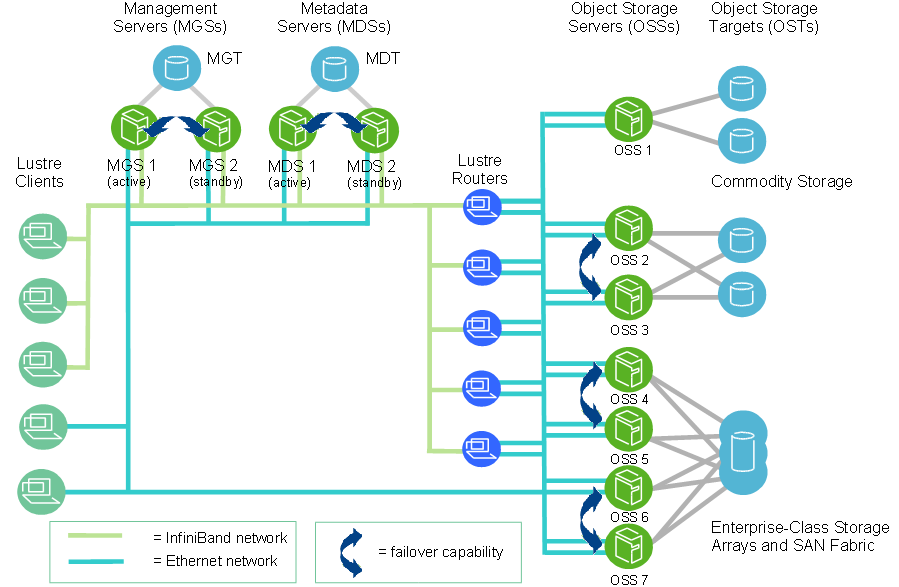
\includegraphics[width=1.0\linewidth]{scaled_cluster}}
\caption{Scaled Cluster}
\label{scaled_cluster}
\end{figure}

À grande échelle, un cluster de système de fichiers Lustre peut inclure des centaines de OSS et des milliers de clients, Figure \ref{scaled_cluster}, Plus d'un type de réseau peut être utilisé dans un cluster Lustre. Le stockage partagé entre OSS permet la fonction de basculement\textit{(failover)}.

\subsubsection{Stockage des données avec Lustre}

	Dans Lustre version 2.0, les identifiants de fichiers Lustre \textit{(File Identifier «FID») }ont été introduites pour remplacer les numéros d'inodes UNIX pour identifier des fichiers ou des objets. Un FID est un identificateur de 128 bits qui contient un numéro unique de 64 bits séquence, un 32-bit ID objet \textit{(Object Identifier «OID»)}, et un numéro de version 32 bits. Le numéro de séquence est unique parmi tous les objectifs Lustre dans un système de fichiers (OST et EMD). Ce changement a permis le soutien futur de plusieurs équipes multidisciplinaires (introduits dans Lustre version 2.3 du logiciel) et ZFS\footnote{http://fr.wikipedia.org/wiki/ZFS}(introduits dans Lustre logiciel version 2.4).\\

\begin{figure}[Donnes en Lustre]
\center{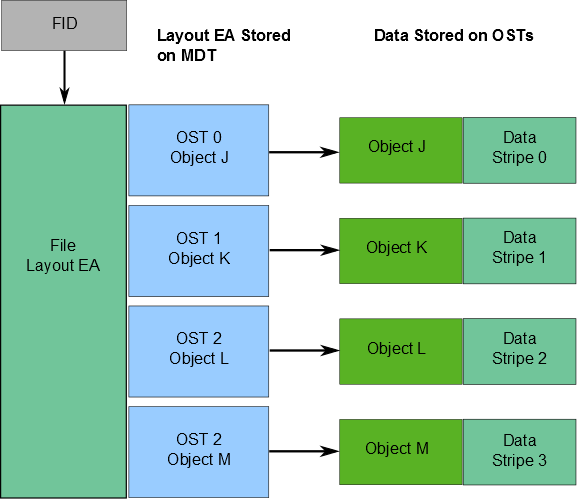
\includegraphics[width=0.5\linewidth]{dataenlustre}}
\caption{Disposition EA sur MDT pointant vers le fichier de données sur OST}
\label{dataenlustre}
\end{figure}

Informations sur l'endroit où les données de fichier se trouve sur le OST, est stockée comme un attribut étendu appelé disposition EA dans un objet MDT identifié par la FID pour le fichier(figure \ref{dataenlustre}). Si le fichier est un fichier de données (pas un répertoire ou un lien symbolique), l'objet MDT pointe de 1 à N OST objet(s) sur le(s) OST(s) qui contiennent les données de fichiers. Si le fichier MDT pointe à un objet, toutes les données de fichier sont stockées dans cet objet. Si le MDT pointe à plus d'un objet, les données du fichier sont réparties sur les objets à l'aide RAID 0, et chaque objet est stocké sur un OST différent.\\

Quand un client veut lire ou écrire dans un fichier, il récupère tout d'abord la mise en EA de l'objet MDT pour le fichier. Le client utilise ensuite ces informations pour effectuer des Entrées/Sorties sur le fichier, interagir directement avec les nœuds OSS où les objets sont stockés(Figure 4).

\begin{figure}[Client-FS]
\center{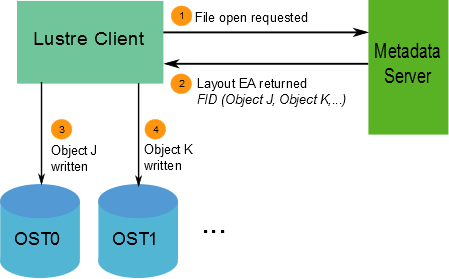
\includegraphics[width=0.6\linewidth]{file_write}}
\caption{Lustre client demandant des données}
\label{fig:identification}
\end{figure}

\newpage
\subsubsection{Lustre et l'entrelacement}

L'un des principaux facteurs menant à la haute performance des systèmes de fichiers Lustre est la capacité de répartir les données sur plusieurs OST dans un mode round-robin. Les utilisateurs peuvent éventuellement configurer pour chaque fichier le nombre de rayures, taille de bande, et OST qui sont utilisés. \\

L'entrelacement\textit{(Striping)} peut être utilisé pour améliorer les performances lorsque la bande passante globale à un fichier unique excède la bande passante d'un seul OST. La capacité de bande est également utile lorsque l'OST n'a pas assez d'espace pour contenir un fichier entier.

Le Stripping permet segments ou «morceaux» de données dans un fichier pour être stocké sur différents OST, dans le système de fichiers Lustre, une configuration RAID 0 est utilisée dans laquelle des données sont «striped» à travers un certain nombre d'objets. Le nombre d'objets dans un seul fichier est appelé \textit{stripe\_count}.

Chaque objet contient un bloc de données à partir du fichier. Lorsque le bloc de données en cours d'écriture à un objet particulier dépasse la \textit{stripe\_size}, le prochain bloc de données dans le fichier est stocké sur l'objet suivant.

Les valeurs par défaut pour \textit{stripe\_count} et \textit{stripe\_size} sont fixés pour le système de fichiers. La valeur par défaut pour \textit{stripe\_count} est une bande de fichier et la valeur par défaut pour \textit{stripe\_size} est 1Mo. L'utilisateur peut modifier ces valeurs sur une base par répertoire ou par fichier.

La taille maximale de fichier n'est pas limité par la taille d'une cible unique. Dans un système de fichiers Lustre, les fichiers peuvent être réparties sur plusieurs objets (jusqu'en 2000), et chaque objet peut être jusqu'à 16 To en taille avec ldiskfs\footnote{http://wiki.lustre.org/lid/ulfi/ulfi\_ldiskfs.html}. Cela conduit à une taille de fichier maximale de 31,25 pétaoctets. (Notez qu'un système de fichiers Lustre peut supporter des fichiers jusqu'à \begin{math}2^{64}\end{math} octets selon le stockage de sauvegarde utilisé par OST.)

\begin{figure}[H]
\center{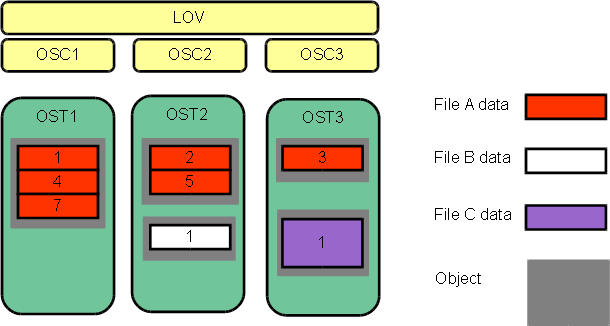
\includegraphics[width=0.6\linewidth]{file_striping}}
\caption{Striping}
\label{fig:identification}
\end{figure}


\newpage
\subsection{Installation}
\subsubsection{CentOS 6.5-Lustre}
Cet essai a était la première fois que nous tentons d’installer Lustre. Le système d'exploitation choisi a été CentOS 6.5. Ce choix s'est tourné ne fut pas très compliqué : c'est un des OS les plus compatibles d'après la documentation, en d'autres mots c'est le système d'exploitation le plus utilisé dans nos tutoriels. Le documentation y est plus importante. Une fois l'ISO téléchargé une autre question se posait. Sur quel support allons-nous déployer le système de fichiers distribués ? En effet, il ne restait plus assez d'ordinateurs dans notre salle de classe. Il faut avouer que nous utilisons déjà 6 machines avec Ceph... Pourquoi ne pas déployer Lustre dessus ? L'installation de ce dernier peut nécessiter des taches assez lourdes comme la compilation du noyau qui peuvent mener à casser le système. Cette situation serait inacceptable, non seulement à cause de Ceph qu'il faudrait réinstaller, mais surtout parce que certaines de ces machines nous servent de machines personnelles pour les cours. Le choix s'est donc tourné vers la virtualisation. Trois machines virtuelles pour être plus précis. Après une rapide lecture de certaines documentations, il s'avère que Lustre est réfléchie de la même manière. C'est à dire qu'il y a aussi les notions de serveurs de stockages et de métadonnées. Nous avons donc décidé d'installer en premier lieu deux serveurs de stockages et un serveur de métadonnées. D'où la mise en place des trois VMs. L'hyperviseur utilisé est KVM, un hyperviseur libre et réputé. Pour gérer et paramétrer les machines virtuelles, nous avons utilisé virt-manager, un outil graphique simple et efficace. Les machines virtuelles ont étés installés en mode minimal sans interface graphique. Chaque VM dispose d'un disque virtuel de 8Go partitionné en deux : 4Go pour CentOS (système + swap) et 4Go de libre pour créer la partition qui servira d'espace de stockage pour le cloud. Les OS nécessites quelques manipulations pour que Lustre ne pose pas de problème. Il faut donc commencer par tuer le service iptables et faire en sorte de ne pas répéter la manipulation à chaque démarrage : 'chkconfig iptables off'. La seconde étape concerne SELinux, un programme qui définit des politiques d'accès à certains éléments de notre système d'exploitation. Voici le fichier de configuration originale:

\begin{figure}[H]
\center{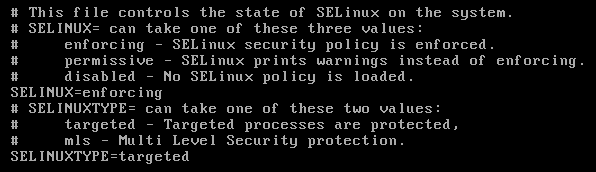
\includegraphics[width=0.6\linewidth]{fig1}}
\caption{Fichier de configuration /etc/sysconfig/selinux par défaut sous CentOS 6.3.}
\label{fig:identification}
\end{figure}


La valeur du paramètre 'SELINUX' doit être affectée à 'permissive' pour que Lustre puisse être installé. Les autres problématiques sont liées aux interfaces réseaux. La première action est utile pour des raisons pratiques. C'est à dire que par défaut, à chaque redémarrage des VMs, il faut démarrer manuellement les interfaces via la commande 'ifup'. Pour changer le comportement par défaut il faut changer l'option ONBOOT à  'yes' dans le fichier de configuration /etc/sysconfig/network-scripts/ifcfg-eth0. La dernière action est liée au clonage des machines virtuelles. En effet, le problème est que ce même fichier, sur le clone, dispose de l'adresse MAC de la machine qui a été clonée et non du clone. Il faut donc changer cette valeur par l'adresse MAC de la VM, disponible via la commande 'ip a'. Après ça, un 'ifup' permet d'avoir accès à internet.

Une fois ces machines virtuelles opérationnelles, il faut aller chercher les sources de Lustre pour notre distribution et plus spécifiquement, il faut choisir les sources adaptées à la version de notre OS et de son noyau. Après une recherche, nous avons les paquets RPM de Lustre adéquats sur ce site : downloads.whamcloud.com. La version précisément choisie est la version lustre-2.5.1 pour el6 pour amd64. Le téléchargement contient des paquets pour le kernel, des paquets pour python et enfin lustre lui-même. Nous nous sommes d'abord contentés de la partie serveur.Maintenant place à l'installation. Pour cela il faut utiliser la commande suivante:

\begin{verbatim}
root@centos63:$rpm -ivh *rpm
\end{verbatim}

Tout de suite, un grand nombre de lignes s'affichaient dans la console. Toutes similaires, c'était des dépendances manquantes. Pas étonnant avec une version minimal du système d'exploitation. Nous avons donc dû installer perl, libatk, libgtk-x11. Après ça, il y avait encore un grand nombre de dépendances non satisfaites. Nous avons donc décidé d'installer paquet par paquet pour s'y retrouver plus facilement, mais aussi pour mieux comprendre les dépendances entre les paquets de Lustre, c'est toujours intéressant. Nous avons donc commencé par installer les paquets liés au noyau. En réglant quelques problèmes de dépendances les paquets se sont installés sans difficultés majeures. Viennent ensuite les paquets python. La prochaine étape va s'avérer un petit peu plus compliquée. C'est donc au tour d'installer les paquets de Lustre. Nous commençons par le paquet contenant les modules du système de fichiers. Problème : il manque ZFS, un système de fichier open source. Pour cela nous avons trouvé une excellente documentation : http://zfsonlinux.org. Nous avons donc importés les archives correspondantes:

\begin{verbatim}
root@centos63:$yum localinstall --nogpgcheck http://archive.zfosonlinux.org/epel/-zfs-release-1.3.ek6.norach.rpm
\end{verbatim}

Il restait ensuite à installer le paquet zfs, avec l'outil yum. Nouvelle tentative pour installer les modules de Lustre : nouvel échec, problème de conflit de kernel. CentOs nous as proposé la désinstallation de ce dernier. Ainsi donc:
\begin{verbatim}
root@centos63:$rpm -e kernel-2.6.32-431.5.5.el6.x86_64
\end{verbatim}

Et:

\begin{verbatim}
root@centos63:$rpm -ivh kernel-2.6.32-358.18.1.el6_lustre.x86_x84.rpm
\end{verbatim}

Aucun problème lors de ces procédures. Ensuite les modules de Lustre se sont installés. C'est maintenant au tour du paquet 'lustre-osd-ldiskfs...' de nous poser des soucis. En effet nous n'avons pas la bonne version d'un programme : e2fsprog. Celui-ci est téléchargeable à l'adresse downloads.whamcloud.com. Maintenant il faut supprimer l'ancienne version et la remplacer par la nouvelle. Il est aussi possible de forcer l'installation directement. Là encore quelques dépendances à résoudre. Toutes les manipulations sont disponibles en annexes. Le paquet Lustre, le cœur du programme, a nécessité également l'installation d'un protocole : snmp. C'est le site net-snmp.sourceforge.net qui héberge le programme.

A ce moment précis, les paquets Lustre server ont étés, à priori, correctement installés sur notre machine virtuelle. Nous avons alors éteint le système dans le but d'en faire un clone comme sauvegarde. Lors du redémarrage de la VM, GNU GRUB, le système d'amorçage, nous a proposé un seul et unique noyau, contre deux initialement après mises à jour:

\begin{figure}[H]
\center{
\includegraphics[width=0.8\linewidth]{fig6}}
\caption{GNU GRUB de la machine virtuelle après installation de Lustre.}
\label{fig:identification}
\end{figure}


Aucune trace de Lustre... Plutôt inquiétant. Ce sentiment a été confirmé lorsque nous avons validé le démarrage sur ce noyau. CentOS ne démarre plus, à la place une erreur : 'Error 15 : File not found'. Nous avons donc eut l'idée de mettre à jour le système d'amorçage. Sur une machine physique, pour ce genre de problème nous démarrons l'ordinateur sur un CDROM ou sur un live USB. L'idée est donc de reproduire la même chose en milieu virtuel. Nous sommes d'abord partis sur un live USB par habitude, mais le périphérique n'était pas présent dans le boot menu. Testons alors l'option du CD.


\begin{figure}[H]
\center{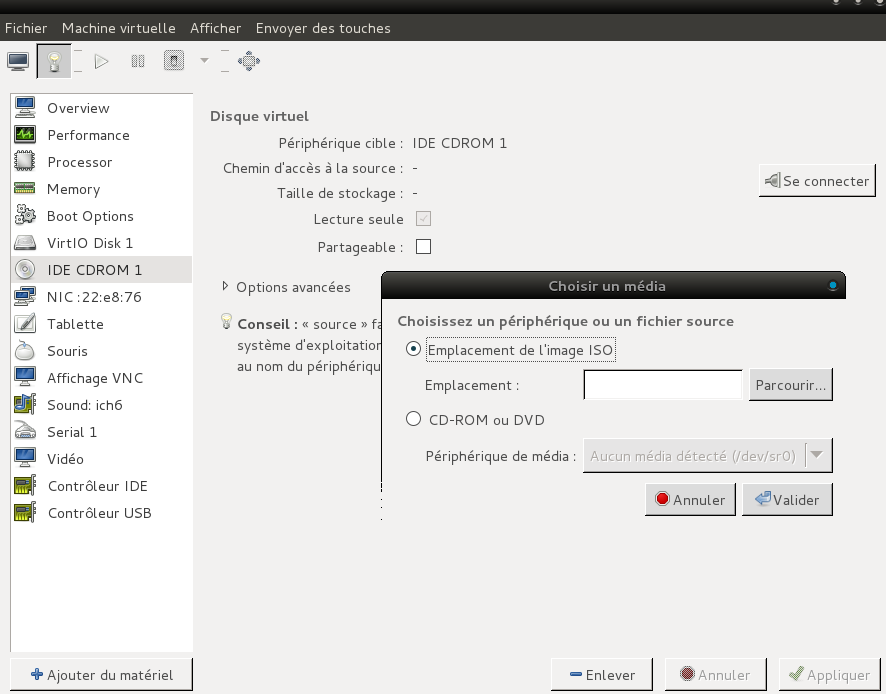
\includegraphics[width=0.8\linewidth]{fig7}}
\caption{Menu virt-manager d'une VM}
\label{fig:identification}
\end{figure}

Pour ajouter un live CD, il faut aller dans les paramètres de la machine virtuelle comme le montre la capture d'écran précédente et sélectionner les options du lecteur CD virtuel. Ensuite il faut cliquer sur le bouton 'Se connecter' à droite de la fenêtre . Enfin la petite fenêtre apparaît et il ne reste plus qu'à indiquer au logiciel l'emplacement de l'image ISO. Nous avons donc réussit à booter en live. Une question se pose : comment mettre à jour le GRUB de notre CentOS ? Pour cela nous sommes connecté à l'OS en chroot. Ainsi nous avons pu lancer la commande 'update-grub'. Nous avons donc redémarrer la machine en faisant attention de bien déconnecter le CD virtuel. Au final, aucun résultat. Toujours le même problème. Il fallait donc changer de méthode.

\newpage
\subsubsection{Ubuntu-Lustre}
Parallèlement à la première tentative d'installation sur CentOS 6.5, en suivant la recommandation de notre tuteur, nous avons décidé de déployer les client Lustre dans une architecture virtualisée, mais en utilisant le système d'exploitation Ubuntu 13.10 cette fois.

Nous avons travaillé également avec KVM et l'outil graphique virt-manager pour créer une machine Virtuelle à laquelle nous avons attribué 7 cpus, 2 Go de mémoire vive et 20 Go de disque dur, cette machine était destinée principalement à la compilation du noyau Linux version 3.13.6, qui donne la possibilité d'activer les drivers compatibles avec Lustre.

Le plan était compiler et installer le nouveau noyau su cette machine et depuis les sources compiler les paquets nécessaires pour l'installation de Lustre sur chaque noeud, cloner la machine 2 fois, réduire ses ressources pour les donner 2 cpus à chacune et 1 Go de mémoire vive, déployer sur les machines clonées et la première machine les clients Lustre.

Nous avons commencé pour la compilation du noyau Linux v13.13.6, la dernière version «stable», nous sommes allés sur le site officiel\footnote{https://www.kernel.org/} pour télécharger les paquets sources.

On a obtenu le fichier «linux-3.13.6.tar.xz» dans notre machine virtuelle, pour extraire le contenu nous avons utilisé la commande:

\begin{verbatim}
	rsmrg@LUT:$tar -Jxvf linux-3.13.6.tar.xz
\end{verbatim}

Ensuite on a changé le répertoire pour nous déplacer vers celui que nous avons extrait du fichier, aussi on a installé les outils de compilation:

\begin{verbatim}
rsmrg@LUT:$cd linux-3.16.6 ; sudo apt-get install debconf-utils dpkg-dev
debhelper  build-essential kernel-package libncurses5-dev
\end{verbatim}

Nous avons copié la configuration du noyau précédant, après on a exécuté, make oldconfig pour répondre aux nouvelles questions de configurations du noyau:

\begin{verbatim}
rsmrg@LUT:$sudo cp /boot/config- 'uname -r' .config
rsmrg@LUT:$make oldconfig
\end{verbatim}

Pour activer les options Lustre on est allé au menu de configuration de noyau dans la partie «Staging drivers» (figure \ref{kernel}).

\begin{verbatim}
rsmrg@LUT:$make menuconfig
\end{verbatim}

\begin{figure}[Lustre Options]
\center{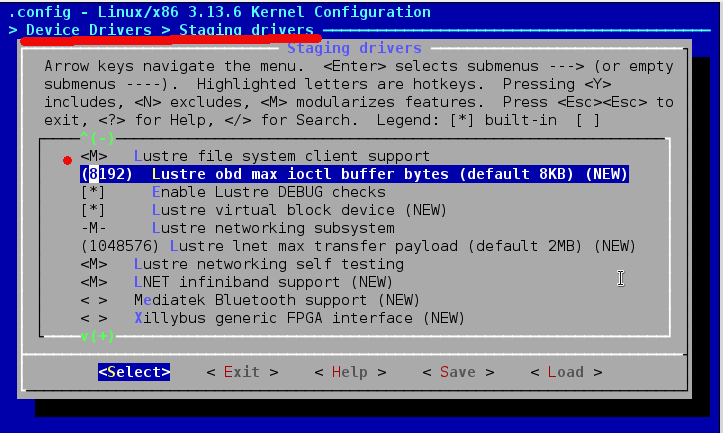
\includegraphics[width=0.8\linewidth]{kernel}}
\caption{Lustre Drivers}
\label{kernel}
\end{figure}

Après sauvegarder les manipulations réalisées, il fallait compiler le noyau en utilisant les 7 cpus et générer les paquets «.deb»:

\begin{verbatim}
rsmrg@LUT:$sudo make -j7 deb-pkg
\end{verbatim}

\begin{figure}[Compilation]
\center{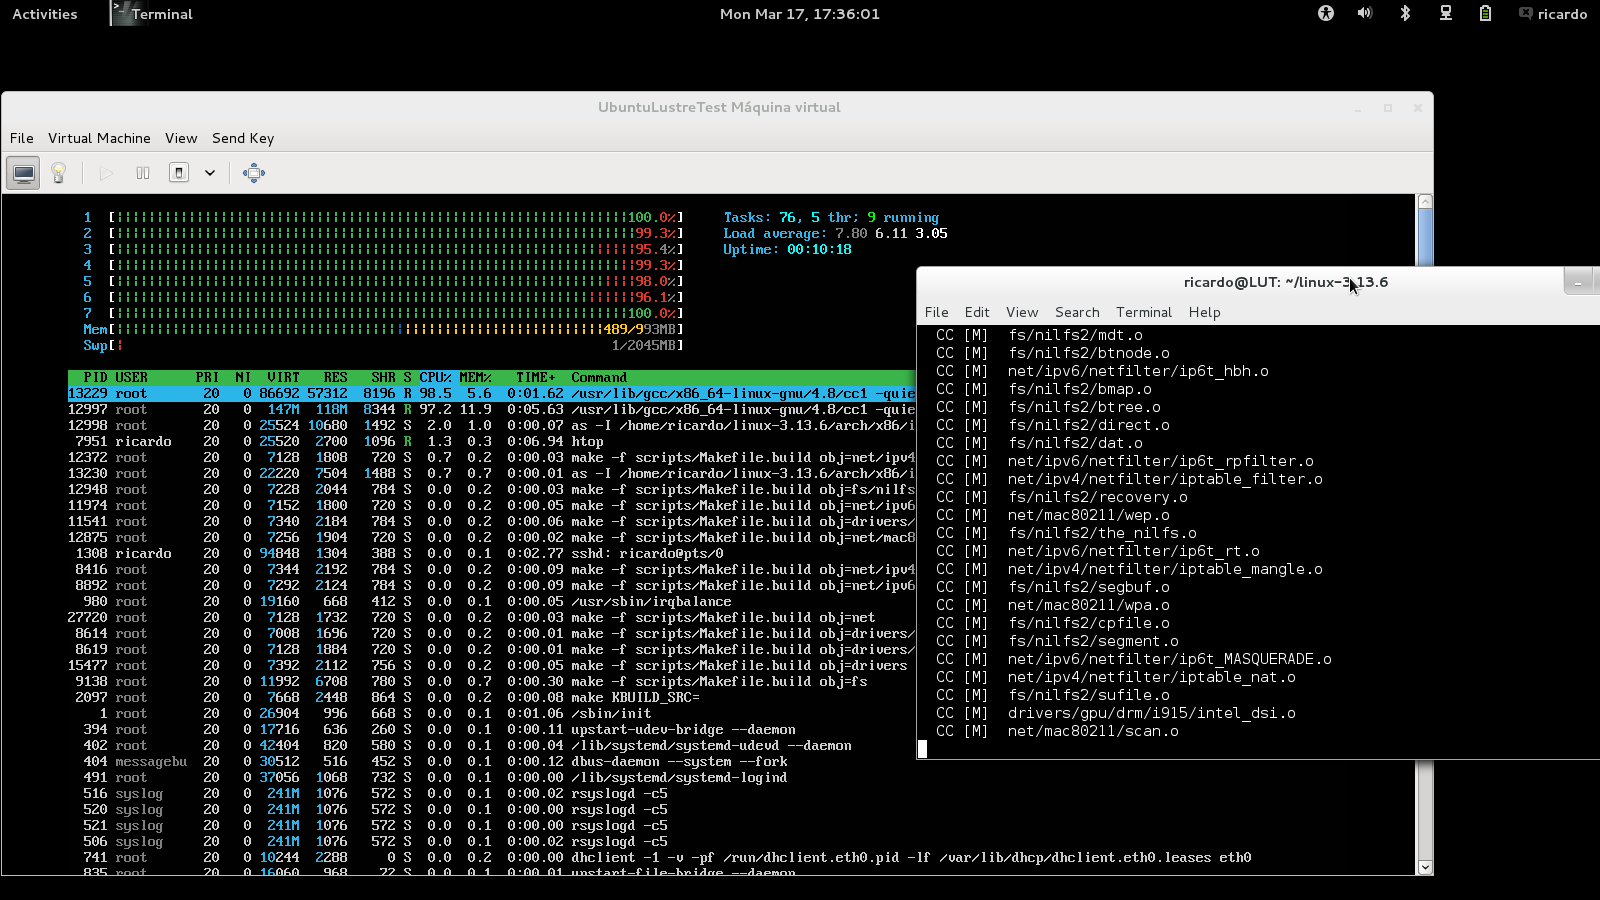
\includegraphics[width=0.8\linewidth]{compilation}}
\caption{Compilation Linux-13.13.6}
\label{kernel}
\end{figure}

Installation du nouveau kernel depuis les paquets généres:

\begin{verbatim}
rsmrg@LUT:$sudo dpkg -i ../*.deb
\end{verbatim}

Après la compilation du noyau de Linux on a essayé d'installer les paquets Lustre sur le système d'exploitation, mais sans succès, après avoir parlé avec le tuteur du projet, il a recommandé l'arrêt de travail avec Ubuntu pour  ne pas perdre plus de temps et de nous consacrer entièrement au déploiement de Lustre avec logiciels plus anciens, mais supportés, comme c'est le cas du système d'exploitation CentOS 6.3.

\newpage
\subsection{CentOS 6.3-Lustre}
C'est la dernière étape pour l'installation de Lustre. Pour cette expérience, le choix s'est reporté à nouveau sur un CentOS. A une différence près. Le version du système d'exploitation utilisé ce coup ci est la version 6.3, au lieu de 6.5 (dernière version stable). La version 6.3 est sensé poser beaucoup moins de soucis en rapport avec le noyau. En effet, l'installation de ce dernier n'est plus nécessaire. Il suffit donc d'installer les paquets RPMs de Lustre. C'est encore une fois Lustre version 2.5 qui est utilisé lors de cette procédure. 

Il faut donc installer une nouvelle fois tous les paquets en réglant les problèmes de dépendance. Tout se passe correctement. Quand, vers la fin de l'installation, des messages d'erreurs apparaissent signifiant que Lustre à besoin d'espace disque... L’exécution de 'df -h' prouve en effet le problème : quelques centaines de MO disponible sur la partition système. En effet par soucis d'espace disque sur la machine physique, la taille des VMs a été revue à la baisse. Elle est passée de 8GO à 6GO. Lors des installations de CentOS en mode minimal, le système d'installation de l'OS ne nous popose qu'un minimum de choix, ce qui veut dire que des choix par défauts sont effectués. Parmi eux, CentOS créé un SWAP, mémoire vive virtuelle, automatiquement. La taille de ce SWAP est proportionnelle à l'espace disponible de la VM, elle représente un certain pourcentage. La répartition de l'espace de stockage de la machine se présente donc ainsi : 4GO pour le système et 2GO pour le SWAP. Récupérer 1GO dans le SWAP afin d'alimenter la partition système serait suffisant sans être handicapant pour l'installation de Lustre. C'est à ce moment que une autre option choisie par la distribution entre en jeu, c'est l'utilisation de LVM pour Logical Volume Manager. LVM est un gestionnaire de volume logique permettant de créer, déplacer, redimensionner et détruire des partitions facilement, sans avoir de problème avec GNU GRUB par exemple. Il est vivement recommandé d'utiliser cette technologie sur des serveurs pour en faciliter la maintenance, les performances n'étant pas beaucoup altérées. CentOS est une distribution optimisée pour une mise ne production sur serveurs, c'est pourquoi ce choix est compréhensible et tout à fait respectable. LVM va donc nous être utile pour diminuer le SWAP et pour augmenter respectivement la partition système. Le redimensionnement à chaud, c'est à dire redimensionner une partition pendant qu'elle est montée, est possible. Seulement vu que il faut manipuler la partition système de l'OS et que nous ne disposons plus assez d'espace libre pour envisager un clone de la machine virtuelle, il est préférable d'assurer le coup et de redimensionner à froid. Pour cela, il a fallu démarrer la machine sur un LiveCD, même iso : CentOS 6.3.

\begin{figure}[H]
\center{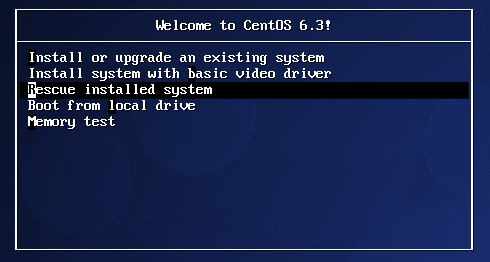
\includegraphics[width=0.8\linewidth]{fig8}}
\caption{Menu d'accueil de CentOS 6.3 en LiveCD}
\label{fig:identification}
\end{figure}

Nous avons choisi de choisir l'option 'Rescue installed system'. Pourquoi le mode 'rescue' ? Parce qu'il permet d'accéder aux outils de LVM, de plus CentOS ne propose pas de mode 'live'. Nous avons fait en sorte que ce mode nous fournisse un shell bash en répondant à quelques questions. Pour analyser les volumes logiques:

\begin{figure}[H]
\center{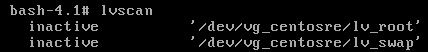
\includegraphics[width=0.8\linewidth]{fig9}}
\caption{Résultat de la commande 'lvscan'}
\label{fig:identification}
\end{figure}

Ainsi donc nous pouvons constater la partie système (/dev/vg\_centosre/lv\_root) et le SWAP(/dev/vg\_centosre/lv\_swap). Place alors au redimensionnement via la commande lvresize qui s'utilise ainsi : 'lvresize -L -1GO /dev/vg\_centosre/lv\_swap' pour le SWAP. Même opération pour la partie système : ' lvresize -L -1GO /dev/vg\_centosre/lv\_swap'. Une fois ces opérations effectuées, il faut redimensionner le système de fichier en fonction de la nouvelle taille de sa partition. Cette opération ne doit pas être pratiquée sur de la mémoire vive virtuelle. Voici la commande a exécuter:

\begin{figure}[H]
\center{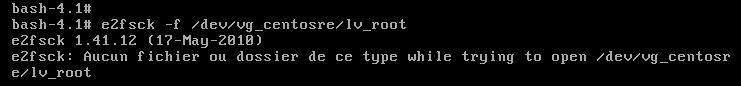
\includegraphics[width=0.8\linewidth]{fig10}}
\caption{Test check système de fichier}
\label{fig:identification}
\end{figure}

Nous voici une nouvelle fois freiné. La commande nous dit qu'elle n'a pas de trouvé la partition. En effet lorsque nous descendons dans l’arborescence, le contenue du dossier /dev ne présente aucun dossier 'vg\_centosre'... Du coup comment faire ? Les commandes 'lvdisplay' et 'vgdisplay' ne nous fournissent pas plus d'informations. Nous avons alors trouvé ne solution simple et rapide : démarrer sur un liveCD, puis monter la partition système de notre CentOS en mode graphique via un gestionnaire de fichiers tel que nautilus ou pcmanfs. Comme vu précédemment, CentOS ne propose pas de mode en live. Il faut donc choisir une autre distribution. Pour cela partons de ce que nous connaissons : nous savons que ubuntu propose le mode live. Seulement celle-ci est devenue lourde, pas optimale pour de la virtualisation avec notre espace disque faible. Nous sommes donc partis sur xubuntu et lubuntu (dans la pratique les deux ont étés testés). Après boot sur LiveCD et montage de la partition racine de notre CentOS, nous avons ouvert une console et avons tapé la commande 'mount'. Résultat, l'emplacement et le nom de la partition recherchée est : /dev/mapper/vg\_centos-lv\_root. Donc nouvel essai avec 'e2fsck' avec le nouveau paramètre. L'opération s'est déroulé sans embûches au premier abord. Donc nous redémarrons notre CentOS et ainsi nous remarquons que la partition avait bien grossi d'un gigaoctet. Parfait, nous voilà prêt pour la suite.

L'installation de Lustre s'est terminé sans autre incident majeur. Une fois cette étape passée, redémarrage de la machine virtuelle. C'est à ce moment que la première installation a posé problème. Un silence s'est ressenti entre nous à ce moment là, tous avions peur d'avoir retenté une manipulation pour rien. Résultat, le menu de démarrage nous propose 3 noyaux, dont celui de Lustre (1ère entrée):

\begin{figure}[H]
\center{
\includegraphics[width=0.8\linewidth]{fig11}}
\caption{GNU GRUB avec le noyau de Lustre.}
\label{fig:identification}
\end{figure}

Excellente nouvelle, CentOS démarre sans incident sur le noyau Lustre. Il reste donc maintenant à déployer les différents nœuds du système de fichiers distribués. Comme énoncé dans le premier test d'installation, nous allons créer trois nœuds. Mais changement de plan. Nous allons mettre en place la structure minimale permettant de pourvoir tester le système le plus rapidement possible. Donc il nous faut un serveur de gestion, un serveur de stockage et un client. Ce changement est né d'un constat : même si l'installation se déroule relativement bien, de nombreux 'warning' apparaissent à l'écran. Ils ne sont pas sensés être problématiques mais sait-on jamais... Nous voulons donc être rassurés impatiemment. La mise en place de ces nœuds se base sur un même principe, celui de formater une partition avec notre système de fichier Lustre. Une fois cette étape validée, il ne reste plus qu'à créer un point de montage. Nous avons décidé que la partition en question serait un disque dur virtuel externe qu'on ajoute via virt-manager:

\begin{figure}[H]
\center{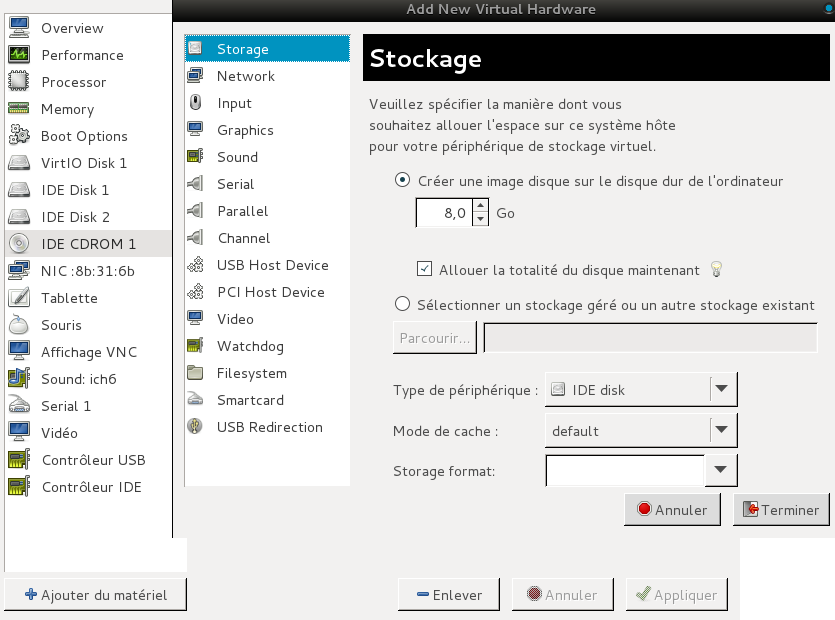
\includegraphics[width=0.8\linewidth]{fig12}}
\caption{Ajout d'un disque dur virtuel externe.}
\label{fig:identification}
\end{figure}

Encore une fois, l'interface de virt-manager se trouve être efficace et simple à la fois. Pour ajouter un matériel, il faut donc cliquer sur le bouton 'Ajouter du matériel' en bas de la fenêtre des options de la machine virtuelle. Ensuite la deuxième fenêtre apparaît où il faut choisir le type de périphérique à ajouter. L'onglet par défaut est 'Storage', celui qui nous concerne. À partir de là il ne reste plus qu'à choisir la taille de cette partition. Les autres options peuvent être laissées par défaut. Dans la capture d'écran précédente, en réalité ce disque est déjà créé : IDE Disk 2. Pour commencer le déploiement de Lustre, c'est le serveur de métadonnée alias MDS ou MGS (le vocabulaire n'est pas toujours le même dans la documentation) qu'il faut d'abord installer. Le MDT est inclus dans cette démarche. Pour retrouver le nom du périphérique qui vient fraîchement d'être installé, l'utilisation de la commande 'fdisk -l' est obligatoire. Ainsi, pour toute nos machines, le disque virtuel se trouve être /dev/sda. Voici donc comment le formater avec Lustre sur notre premier serveur:

\begin{figure}[H]
\center{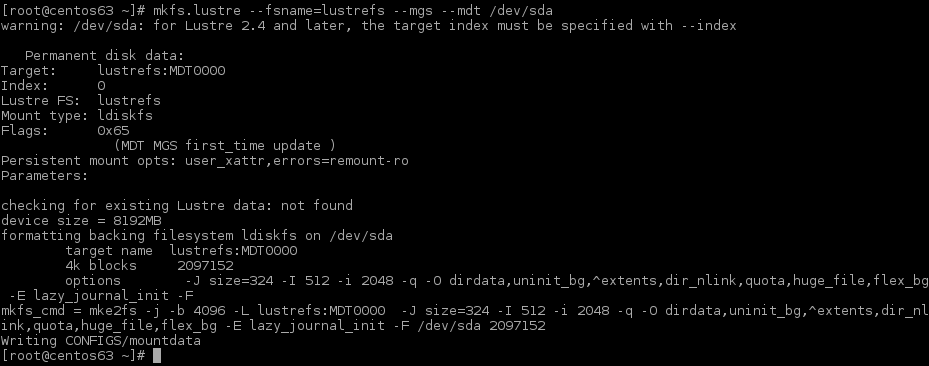
\includegraphics[width=0.8\linewidth]{fig13}}
\caption{Installation de système de fichier Lustre.}
\label{fig:identification}
\end{figure}

Et voici comment monter cet élément:

\begin{figure}[H]
\center{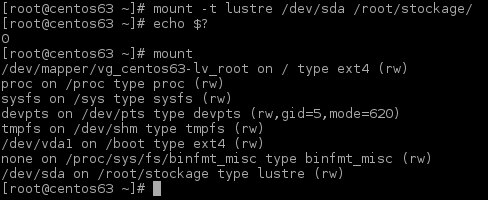
\includegraphics[width=0.8\linewidth]{fig14}}
\caption{Création d'un point d'accès de la partition Lustre.}
\label{fig:identification}
\end{figure}

Mise en place de l'OST de la même manière:

\begin{figure}[H]
\center{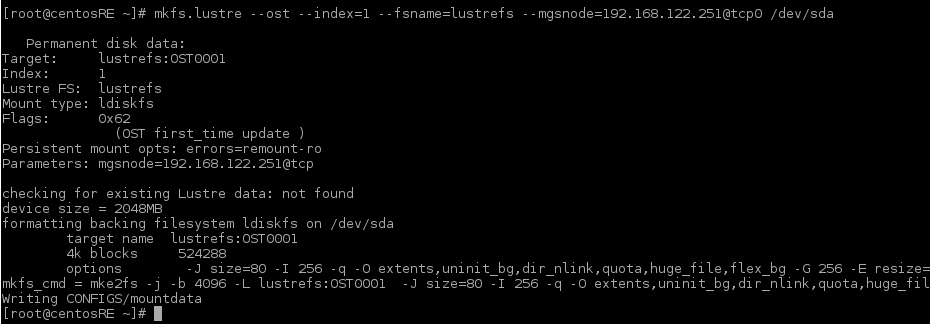
\includegraphics[width=0.8\linewidth]{fig15}}
\caption{Installation de système de fichier Lustre.}
\label{fig:identification}
\end{figure}

Il est bon de remarquer que la grappe de serveurs se déploie pratiquement comme Ceph. Pour Ceph, toute l'installation se fait à partir d'un nœud principal. Ici, l'installation se fait sur chaque machine mais l'adresse ip du premier nœud doit quand même être fourni. La procédure n'est pas la même, mais le fonctionnement des deux systèmes est similaire. Il faut aussi monter l'espace de stockage:

\begin{figure}[H]
\center{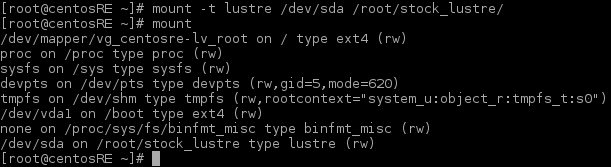
\includegraphics[width=0.8\linewidth]{fig16}}
\caption{Création d'un point d'accès de la partition Lustre.}
\label{fig:identification}
\end{figure}

La procédure est donc fini pour le serveur de stockage. Il faut maintenant s'occuper du client. La seule étape nécessaire est de monter le système de fichiers:

\begin{figure}[H]
\center{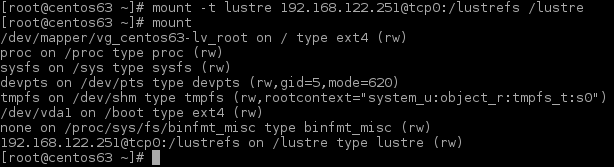
\includegraphics[width=0.8\linewidth]{fig17}}
\caption{Création d'un point d'accès de la partition Lustre.}
\label{fig:identification}
\end{figure}

Nous voyons bien que l'opération s'est exécutée correctement, le client est bel et bien en place. La partition monté sur /lustre est accessible par le réseau via l'adresse ip de notre serveur de métadonnées comme prévus. Attention cette ligne (dernière ligne retournée par 'mount' sur la figure ci-dessus) peut faire penser à la syntaxe utilisée par la commande 'scp', la copie de données via SSH. C'est à dire que la partie '/lustrefs' ne représente pas un dossier disponible à l'adresse ip correspondante, mais précise le cluster Lustre. Nous avons fourni ce nom dans les commandes précédentes lors du formatage des disques virtuels. 


\subsection{Conclusion}
\subsection{Lustre}
\subsection{Faru}


http://doc.ubuntu-fr.org/tutoriel/compiler\_linux 
http://wiki.lustre.org/manual/LustreManual18\_HTML/IntroductionToLustre.html
http://wiki.lustre.org/index.php/Debian\_Install
https://wiki.debian.org/Lustre
http://downloads.whamcloud.com/public/lustre/lustre-2.5.1/el6/client/RPMS/x86\_64/
http://ocubom.wordpress.com/2008/05/21/estructuras-basicas-de-latex/
http://en.wikipedia.org/wiki/Lustre\_(file\_system)

\end{document}
